% Ajuste fino de modelos pré-treinados para uma tarefa
% Compilar dentro de slides/:  latexmk -pdf apresentacao.tex
% Figuras: ../results/figuras/ (geradas por code/gerar_figuras.py)
% Números: ../results/tabela_resultados.md e docs/referencias.md

\documentclass[aspectratio=169,10pt]{beamer}

\usepackage[utf8]{inputenc}
\usepackage[T1]{fontenc}
\usepackage[brazil]{babel}
\usepackage[sfdefault,lining]{FiraSans}
\usepackage[scale=0.85]{FiraMono}
\usepackage{booktabs}
\usepackage{array}
\newcolumntype{L}[1]{>{\raggedright\arraybackslash}p{#1}}
\usepackage{graphicx}
\usepackage{listings}
\usepackage{tikz}
\usetikzlibrary{positioning,arrows.meta,shapes.misc}

\usetheme[progressbar=frametitle,numbering=fraction,sectionpage=progressbar]{metropolis}

% Cores iguais às das figuras
\definecolor{azul}{HTML}{2A78D6}
\definecolor{laranja}{HTML}{EB6834}
\definecolor{tinta}{HTML}{0B0B0B}
\definecolor{tinta2}{HTML}{52514E}
\definecolor{fundocod}{HTML}{F4F3F0}
\setbeamercolor{frametitle}{bg=tinta, fg=white}
\setbeamercolor{progress bar}{fg=azul, bg=azul!20}
\setbeamercolor{alerted text}{fg=laranja}
\setbeamercolor{example text}{fg=azul}
\setbeamercolor{normal text}{fg=tinta}

\graphicspath{{../results/figuras/}}

\lstset{
  language=Python,
  basicstyle=\ttfamily\footnotesize,
  keywordstyle=\color{azul}\bfseries,
  stringstyle=\color{laranja!80!black},
  commentstyle=\color{tinta2}\itshape,
  backgroundcolor=\color{fundocod},
  frame=none,
  xleftmargin=4pt, xrightmargin=4pt,
  aboveskip=4pt, belowskip=4pt,
  showstringspaces=false,
  columns=fullflexible,
  keepspaces=true,
  upquote=true,
  literate={á}{{\'a}}1 {à}{{\`a}}1 {ã}{{\~a}}1 {â}{{\^a}}1 {é}{{\'e}}1 {ê}{{\^e}}1
           {í}{{\'i}}1 {ó}{{\'o}}1 {õ}{{\~o}}1 {ô}{{\^o}}1 {ú}{{\'u}}1 {ç}{{\c{c}}}1
           {Ç}{{\c{C}}}1 {É}{{\'E}}1 {Ê}{{\^E}}1 {Ã}{{\~A}}1 {Á}{{\'A}}1 {Í}{{\'I}}1
           {Ó}{{\'O}}1 {Õ}{{\~O}}1 {Ú}{{\'U}}1 {→}{{$\to$}}1,
}

\newcommand{\fonte}[1]{\par\vfill{\scriptsize\color{tinta2}Fonte: #1}}
\newcommand{\destaque}[1]{{\color{azul}\bfseries #1}}

\title{Ajuste fino de modelos pré-treinados}
\subtitle{Adaptando o BERTimbau para classificar o sentimento de avaliações}
\author{Wagner Aladiah Pacheco de Almeida}
\institute{Universidade Federal de Alagoas (UFAL)\\ Processamento de Linguagem Natural, Prof.\ Thales Vieira}
\date{27 de novembro de 2026}

\begin{document}

\maketitle

% ===================================================================
% Bloco 1: abertura (1 min)
% ===================================================================

\begin{frame}{Treinar do zero ou reaproveitar?}
  \begin{columns}[T]
    \begin{column}{0.48\textwidth}
      \textbf{Treinar do zero para cada tarefa}
      \begin{itemize}
        \item muitos dados rotulados
        \item muito processamento
        \item o modelo aprende a língua \emph{e} a tarefa ao mesmo tempo
      \end{itemize}
    \end{column}
    \begin{column}{0.48\textwidth}
      \textbf{Ajuste fino}
      \begin{itemize}
        \item aprender a língua uma vez, com texto \emph{sem} rótulo
        \item adaptar a cada tarefa com \destaque{poucos} exemplos rotulados
        \item é transferência de aprendizado: o que vale para uma tarefa ajuda a outra
      \end{itemize}
    \end{column}
  \end{columns}
  \vspace{0.5em}
  \begin{center}
    Pergunta desta apresentação: \alert{como se adapta um modelo pré-treinado a uma tarefa,\\ e quando essa adaptação deixa de generalizar?}
  \end{center}
\end{frame}

% ===================================================================
% Bloco 2: fundamentos (6 min)
% ===================================================================

\section{Fundamentos}

\begin{frame}{Duas fases: pré-treino e ajuste fino}
  \centering
  \begin{tabular}{@{}L{0.13\textwidth}L{0.41\textwidth}L{0.38\textwidth}@{}}
    \toprule
    & \textbf{Pré-treino} & \textbf{Ajuste fino} \\
    \midrule
    Dados & muito texto \emph{sem} rótulo & poucos exemplos \emph{rotulados} \\
    Objetivo & prever palavras mascaradas (sem rótulo humano) & a tarefa: positivo ou negativo \\
    Quem faz & quem publica o modelo (NeuralMind, no BERTimbau) & nós \\
    Custo & alto: dias de TPU/GPU & baixo: \destaque{4 min} numa GPU gratuita \\
    Resultado & pesos genéricos do encoder & encoder ajustado + cabeça da tarefa \\
    \bottomrule
  \end{tabular}
  \vspace{1em}

  \begin{quote}
    \small O modelo pré-treinado ``pode ser ajustado com apenas uma camada de saída adicional'' para várias tarefas, ``sem modificações substanciais na arquitetura''.
  \end{quote}
  \fonte{Devlin et al. (2019), BERT [1]; custo do ajuste fino: experimento E2 deste trabalho.}
\end{frame}

\begin{frame}{O que muda no modelo}
  \centering
  \begin{tikzpicture}[
      node distance=7mm,
      caixa/.style={rounded rectangle, draw=tinta2, thick, minimum height=8mm, inner xsep=7pt, font=\small},
      nova/.style={caixa, draw=laranja, fill=laranja!12},
      pre/.style={caixa, draw=azul, fill=azul!10},
      seta/.style={-{Stealth[length=2.5mm]}, thick, tinta2},
      rot/.style={font=\scriptsize, text=tinta2}]
    \node[caixa] (texto) {``Chegou rápido e funciona''};
    \node[caixa, right=20mm of texto, font=\scriptsize\ttfamily] (tok) {[CLS] Chegou ... [SEP]};
    \node[pre, right=of tok] (enc) {encoder: 12 camadas};
    \node[pre, below=9mm of enc] (cls) {vetor do \texttt{[CLS]} (768)};
    \node[nova, left=12mm of cls] (cab) {cabeça: 768 $\to$ 2};
    \node[caixa, left=12mm of cab] (prob) {softmax: 97\% positivo};
    \draw[seta] (texto) -- node[rot, above]{tokenizador} (tok);
    \draw[seta] (tok) -- (enc);
    \draw[seta] (enc) -- (cls);
    \draw[seta] (cls) -- (cab);
    \draw[seta] (cab) -- (prob);
    \node[rot, above=1mm of enc] {pré-treinado};
    \node[rot, below=1mm of cab, text=laranja] {nova, pesos aleatórios};
  \end{tikzpicture}
  \vspace{1.2em}

  \begin{columns}[T]
    \begin{column}{0.45\textwidth}
      \centering
      {\Large\color{azul}\textbf{108.924.674}}\\
      parâmetros ajustados (todos)
    \end{column}
    \begin{column}{0.45\textwidth}
      \centering
      {\Large\color{laranja}\textbf{1.538}}\\
      parâmetros novos (só a cabeça)
    \end{column}
  \end{columns}
  \fonte{\texttt{results/e2\_ajuste\_completo/parametros.json}. A probabilidade do diagrama é ilustrativa.}
\end{frame}

\begin{frame}{Como o treino funciona}
  \begin{columns}[T]
    \begin{column}{0.5\textwidth}
      \textbf{Perda: entropia cruzada}
      \[
        L = -\log p_{\text{correta}}
      \]
      \[
        p = \operatorname{softmax}(W\,h_{\texttt{[CLS]}} + b)
      \]
      \begin{itemize}
        \item o gradiente passa pela cabeça e por \destaque{todas} as camadas do encoder
        \item taxa de aprendizado \destaque{pequena}, para não apagar o que o pré-treino ensinou
      \end{itemize}
    \end{column}
    \begin{column}{0.45\textwidth}
      \textbf{Faixa sugerida pelo BERT}
      \begin{itemize}
        \item batch: 16 ou 32
        \item taxa (Adam): 5e-5, 3e-5 ou 2e-5
        \item épocas: 2, 3 ou 4
        \item dropout: 0,1
      \end{itemize}
      \vspace{0.5em}
      Conjuntos grandes (100 mil+ exemplos) são bem menos sensíveis a essa escolha.
    \end{column}
  \end{columns}
  \fonte{Devlin et al. (2019), apêndice A.3 [1].}
\end{frame}

\begin{frame}{Variações e por que funciona com poucos dados}
  \begin{columns}[T]
    \begin{column}{0.52\textwidth}
      \small
      \begin{tabular}{@{}L{0.5\linewidth}L{0.46\linewidth}@{}}
        \toprule
        \textbf{Variação} & \textbf{O que treina} \\
        \midrule
        Ajuste fino completo & encoder + cabeça \emph{(este trabalho)} \\
        Extração de características (encoder congelado) & só a cabeça \\
        Descongelamento gradual & camadas liberadas aos poucos \\
        Ajuste eficiente (LoRA etc.) & poucos parâmetros extras \\
        \bottomrule
      \end{tabular}
    \end{column}
    \begin{column}{0.43\textwidth}
      \textbf{ULMFiT (2018)}
      \begin{itemize}
        \item erro \destaque{18--24\% menor} na maioria de 6 conjuntos de classificação
        \item com \destaque{100 exemplos} rotulados, igualou treinar do zero com \destaque{100 vezes} mais dados
      \end{itemize}
      \vspace{0.5em}
      O pré-treino já entrega representações úteis; o ajuste fino só as ``aponta'' para a tarefa.
    \end{column}
  \end{columns}
  \fonte{Howard e Ruder (2018), ULMFiT [2], resumo.}
\end{frame}

% ===================================================================
% Bloco 3: código, preparação dos dados (3 min)
% ===================================================================

\section{O código}

\begin{frame}{O exemplo: sentimento em avaliações de produtos}
  \begin{columns}[T]
    \begin{column}{0.5\textwidth}
      \begin{itemize}
        \item \textbf{Modelo:} BERTimbau base, um BERT pré-treinado em português\\ {\scriptsize\texttt{neuralmind/bert-base-portuguese-cased}}
        \item \textbf{Dados:} B2W-Reviews01, avaliações de uma loja on-line, nota de 1 a 5
        \item \textbf{Tarefa:} positivo × negativo
        \item \textbf{Código:} \texttt{transformers} + \texttt{datasets}, Colab com GPU T4
      \end{itemize}
    \end{column}
    \begin{column}{0.45\textwidth}
      \small
      \begin{tabular}{@{}ll@{}}
        \toprule
        \textbf{Exp.} & \textbf{Pergunta} \\
        \midrule
        E1 & quanto acerta sem ajuste fino? \\
        E2 & e com ajuste fino completo? \\
        E3 & como o sobreajuste aparece? \\
        E4 & early stopping ajuda? \\
        E5 & generaliza para outro domínio? \\
        E6 & quantos exemplos são precisos? \\
        \bottomrule
      \end{tabular}
    \end{column}
  \end{columns}
  \fonte{Souza et al. (2020) [3]; Real et al. (2019) [8]; código em \texttt{code/ajuste\_fino.py}.}
\end{frame}

\begin{frame}[fragile]{Preparação dos dados: do texto ao rótulo}
  \begin{lstlisting}
# [PREPARAÇÃO DOS DADOS] limpeza e rótulo binário
ds = bruto.filter(
    lambda ex: ex["review_text"] is not None
    and ex["review_text"].strip() != ""
    and ex["overall_rating"] != 3
)
ds = ds.map(
    lambda ex: {"texto": ex["review_text"].strip(), "label": int(ex["overall_rating"] >= 4)},
    remove_columns=ds.column_names,
)
tabela = ds.to_pandas().drop_duplicates(subset="texto")
  \end{lstlisting}
  \begin{itemize}
    \item nota 1--2 $\to$ \textbf{negativo}; 4--5 $\to$ \textbf{positivo}; nota 3 é ambígua e \alert{sai}
    \item duplicatas saem: uma cópia no treino e outra no teste inflaria a métrica
    \item 132.373 avaliações $\to$ \destaque{110.882} depois da limpeza; 70,6\% positivas
  \end{itemize}
  \fonte{\texttt{results/e2\_ajuste\_completo/dados.json}.}
\end{frame}

\begin{frame}[fragile]{Preparação dos dados: divisão e tokenização}
  \begin{columns}[T]
    \begin{column}{0.48\textwidth}
      \textbf{Três conjuntos, três papéis}
      \begin{itemize}
        \item \textbf{treino} (80\%): ajusta os pesos
        \item \textbf{validação} (10\%): escolhe a época, decide o early stopping
        \item \textbf{teste} (10\%, 11.089): usado uma vez, no fim
      \end{itemize}
      Divisão estratificada e com semente fixa: todos os experimentos usam o mesmo teste.
    \end{column}
    \begin{column}{0.48\textwidth}
      \textbf{Tokenização (WordPiece)}\\[2pt]
      \small ``Produto confortável, ajusta bem ao bebê e não machuca \dots''\\[4pt]
      {\raggedright\ttfamily\scriptsize
      \colorbox{azul!15}{[CLS]} Produ \colorbox{laranja!20}{\#\#to} confor \colorbox{laranja!20}{\#\#tável} , ajus \colorbox{laranja!20}{\#\#ta} bem ao bebê e não machu \colorbox{laranja!20}{\#\#ca} \dots{} \colorbox{azul!15}{[SEP]}\par}
      \begin{itemize}
        \item vocabulário fixo de 29.794 subpalavras
        \item corte em 128 tokens: mediana de 26, só 2,4\% truncados
        \item padding por lote (\texttt{DataCollatorWithPadding})
      \end{itemize}
    \end{column}
  \end{columns}
  \fonte{\texttt{results/e2\_ajuste\_completo/tokenizacao.json}.}
\end{frame}

% ===================================================================
% Bloco 4: código, treinamento (4 min)
% ===================================================================

\begin{frame}[fragile]{Treinamento: o modelo e os hiperparâmetros}
  \begin{columns}[T]
    \begin{column}{0.55\textwidth}
      \begin{lstlisting}[basicstyle=\ttfamily\scriptsize]
# [TREINAMENTO] encoder pré-treinado
# + camada de classificação nova
modelo = AutoModelForSequenceClassification\
    .from_pretrained(MODELO, num_labels=2, ...)

argumentos = TrainingArguments(
    num_train_epochs=2,
    learning_rate=2e-5,
    per_device_train_batch_size=32,
    weight_decay=0.01,
    warmup_steps=int(0.1 * passos_total),
    lr_scheduler_type="linear",
    fp16=True,
    ...
)
      \end{lstlisting}
    \end{column}
    \begin{column}{0.42\textwidth}
      \small
      \begin{itemize}
        \item \textbf{taxa 2e-5}: dentro da faixa do BERT
        \item \textbf{2 épocas}: mais épocas aumentam o risco de sobreajuste
        \item \textbf{aquecimento}: a taxa sobe de 0 nos 10\% iniciais, enquanto a cabeça ainda é aleatória
        \item \textbf{weight decay}: puxa os pesos para perto de zero
        \item \textbf{fp16}: meia precisão, mais rápido
      \end{itemize}
    \end{column}
  \end{columns}
  \fonte{\texttt{code/ajuste\_fino.py}, função \texttt{treinar} (trecho simplificado).}
\end{frame}

\begin{frame}[fragile]{Treinamento: o que o \texttt{Trainer} faz}
  \begin{columns}[T]
    \begin{column}{0.5\textwidth}
      \begin{lstlisting}
trainer = Trainer(
    model=modelo,
    args=argumentos,
    train_dataset=treino_tok,
    eval_dataset=validacao_tok,
    data_collator=DataCollatorWithPadding(tok),
    compute_metrics=calcular_metricas,
)
trainer.train()
      \end{lstlisting}
      \small Métrica: \textbf{F1 macro}. Chutar sempre ``positivo'' dá 70,6\% de acurácia, mas só 41,4\% de F1 macro.
    \end{column}
    \begin{column}{0.45\textwidth}
      A cada passo:
      \begin{enumerate}
        \item monta um lote com padding
        \item calcula os logits
        \item calcula a entropia cruzada
        \item retropropaga por \destaque{todas} as camadas
        \item atualiza os pesos (AdamW) e a taxa
        \item de tempos em tempos, avalia na validação
      \end{enumerate}
      \vspace{0.3em}
      \textbf{Custo (E2):} \destaque{242 s} e \destaque{3,01 GB} de GPU (de 15 GB da T4)
    \end{column}
  \end{columns}
  \fonte{\texttt{results/e1\_referencia/metricas.json}; \texttt{results/e2\_ajuste\_completo/metricas.json}.}
\end{frame}

% ===================================================================
% Bloco 5: código, inferência (2 min)
% ===================================================================

\begin{frame}[fragile]{Inferência: classificando textos novos}
  \begin{columns}[T]
    \begin{column}{0.38\textwidth}
      \begin{lstlisting}[basicstyle=\ttfamily\scriptsize]
# [INFERÊNCIA] modelo salvo pelo E2
modelo = AutoModelForSequence\
    Classification.from_pretrained(pasta)
tok = AutoTokenizer.from_pretrained(pasta)

classificar = pipeline(
    "text-classification",
    model=modelo, tokenizer=tok)
classificar(frases)
      \end{lstlisting}
      \footnotesize O \texttt{pipeline} tokeniza com o \alert{mesmo} tokenizador do treino, roda o modelo e aplica softmax.
    \end{column}
    \begin{column}{0.6\textwidth}
      \scriptsize
      \renewcommand{\arraystretch}{1.15}
      \begin{tabular}{@{}L{0.64\linewidth}lr@{}}
        \toprule
        \textbf{Frase} & \textbf{Previsto} & \textbf{Prob.} \\
        \midrule
        Chegou antes do prazo e funciona perfeitamente. & positivo & 99,9\% \\
        Não recomendo, quebrou na primeira semana. & negativo & 99,1\% \\
        O filme é longo, mas vale cada minuto. & positivo & 99,4\% \\
        O atendimento do restaurante foi péssimo. & negativo & 87,2\% \\
        Não é ruim. & positivo & 60,7\% \\
        Esperava mais pelo preço que paguei. & negativo & 77,5\% \\
        \midrule
        \textcolor{laranja}{Ótimo, mais um carregador que não carrega.} & \textcolor{laranja}{positivo} & \textcolor{laranja}{99,6\%} \\
        \textcolor{laranja}{A entrega foi feita na terça-feira.} & \textcolor{laranja}{positivo} & \textcolor{laranja}{72,7\%} \\
        \bottomrule
      \end{tabular}
      \par\vspace{4pt}
      \small Ironia errada com \alert{99,6\%}; frase neutra forçada a ``positivo'' (a nota 3 saiu na preparação).
    \end{column}
  \end{columns}
  \fonte{\texttt{results/e5\_generalizacao/frases\_novas.json}.}
\end{frame}

% ===================================================================
% Bloco 6: exemplo e resultados (4 min)
% ===================================================================

\section{Resultados}

\begin{frame}{O ajuste fino contra as referências}
  \centering
  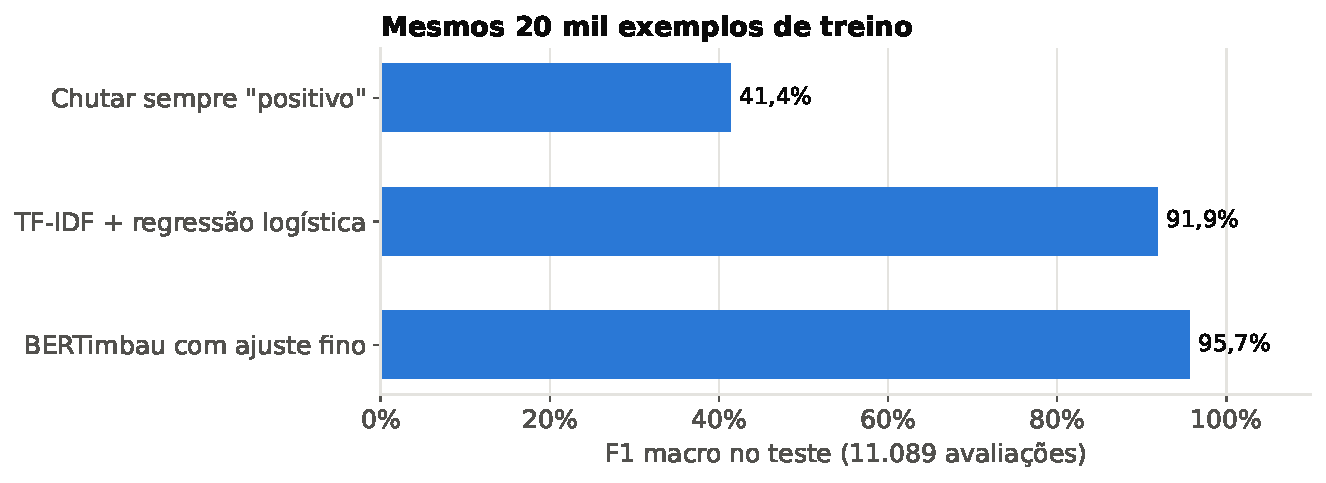
\includegraphics[width=0.78\textwidth]{comparacao_metodos.pdf}
  \begin{itemize}
    \item o modelo clássico é forte, mas o ajuste fino \destaque{quase reduz o erro à metade}: de 6,7\% para 3,6\% (acurácia 93,3\% $\to$ 96,4\%)
    \item mesmos 20 mil exemplos de treino e mesmo teste de 11.089 avaliações
  \end{itemize}
  \fonte{E1 e E2; \texttt{results/tabela\_resultados.md}.}
\end{frame}

\begin{frame}{Quantos exemplos rotulados são precisos?}
  \begin{columns}[c]
    \begin{column}{0.62\textwidth}
      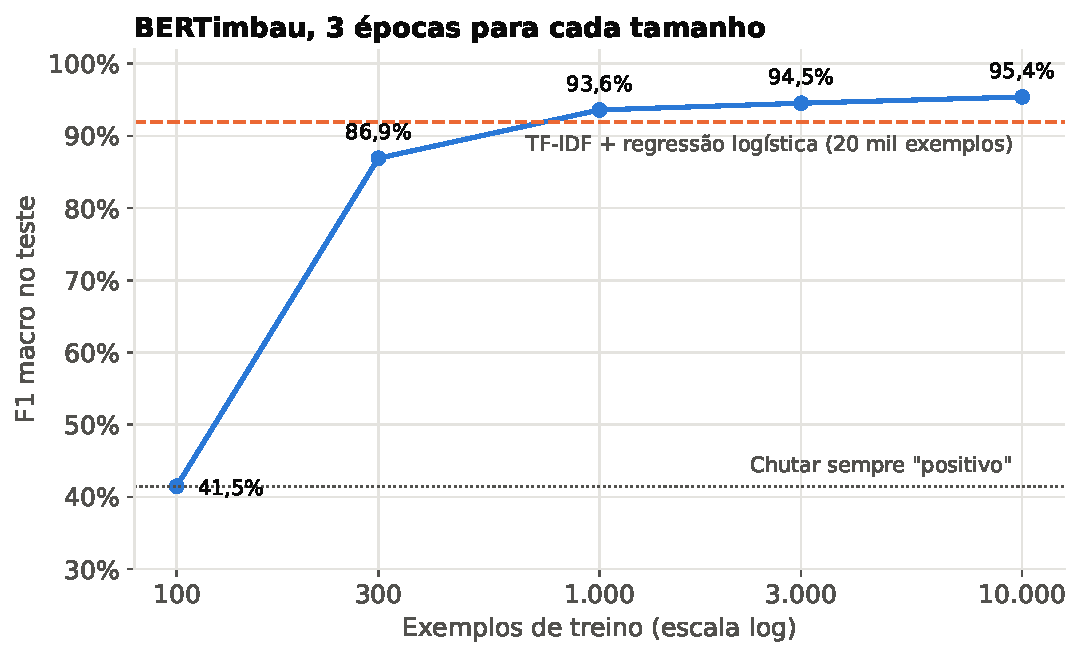
\includegraphics[width=\textwidth]{curva_aprendizado.pdf}
    \end{column}
    \begin{column}{0.36\textwidth}
      \begin{itemize}
        \item com \destaque{1.000} exemplos, o BERTimbau supera o TF-IDF com \destaque{20.000}
        \item de 1.000 para 10.000 (10 vezes mais), o F1 sobe só 1,8 ponto
        \item com 100 exemplos, não sai do chute: são só 12 atualizações dos pesos
      \end{itemize}
      \small O mesmo efeito do ULMFiT, agora em português.
    \end{column}
  \end{columns}
  \fonte{E6 e E1; \texttt{results/tabela\_resultados.md}.}
\end{frame}

% ===================================================================
% Bloco 7: sobreajuste e generalização (3 min)
% ===================================================================

\section{Sobreajuste e generalização}

\begin{frame}{Sobreajuste: o modelo decora o treino}
  \begin{columns}[c]
    \begin{column}{0.58\textwidth}
      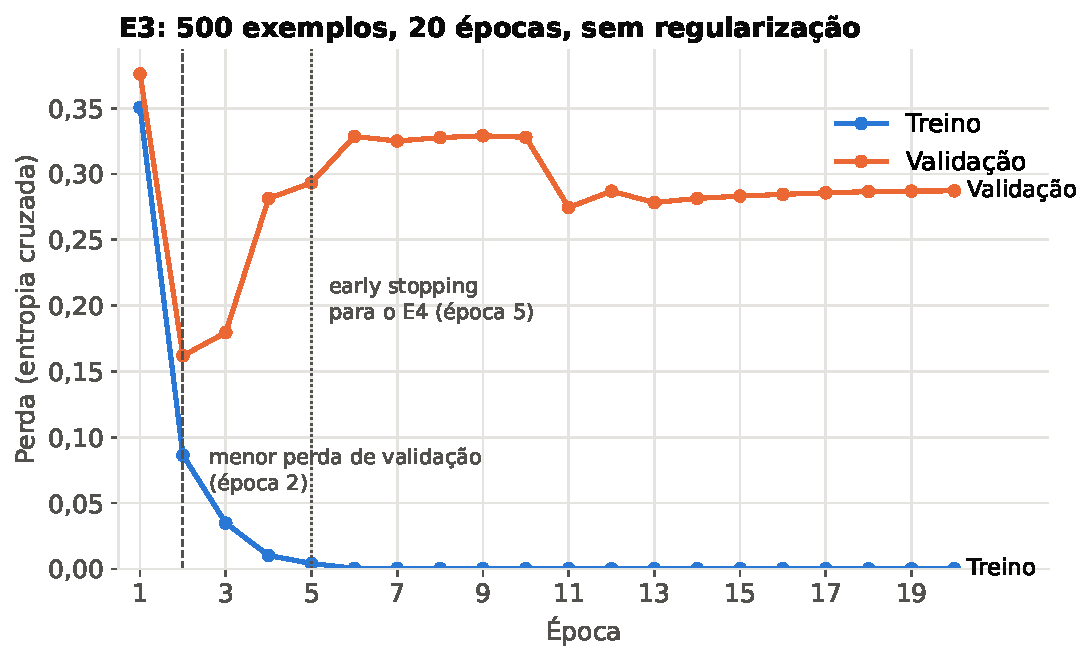
\includegraphics[width=\textwidth]{curva_sobreajuste.pdf}
    \end{column}
    \begin{column}{0.4\textwidth}
      \small
      \begin{itemize}
        \item treino chega a \alert{100\%} de acurácia; a validação é melhor na época 2 e depois piora
        \item a perda sobe, mas o F1 fica entre 92,5\% e 95,1\%: o modelo continua acertando, mas fica \alert{confiante demais quando erra}
      \end{itemize}
      \scriptsize
      \begin{tabular}{@{}lrr@{}}
        \toprule
        & \textbf{E3} & \textbf{E4 (early stop.)} \\
        \midrule
        Épocas & 20 & 5 (usa a 2ª) \\
        F1 no teste & 93,6\% & 93,4\% \\
        Perda no teste & 0,361 & \destaque{0,166} \\
        Tempo & 150 s & \destaque{85 s} \\
        \bottomrule
      \end{tabular}
    \end{column}
  \end{columns}
  \fonte{E3 e E4, 500 exemplos; \texttt{results/e3\_sobreajuste/}, \texttt{results/e4\_regularizado/}. Uma semente por experimento.}
\end{frame}

\begin{frame}{Generalização: mesma tarefa, outro domínio}
  \begin{columns}[c]
    \begin{column}{0.55\textwidth}
      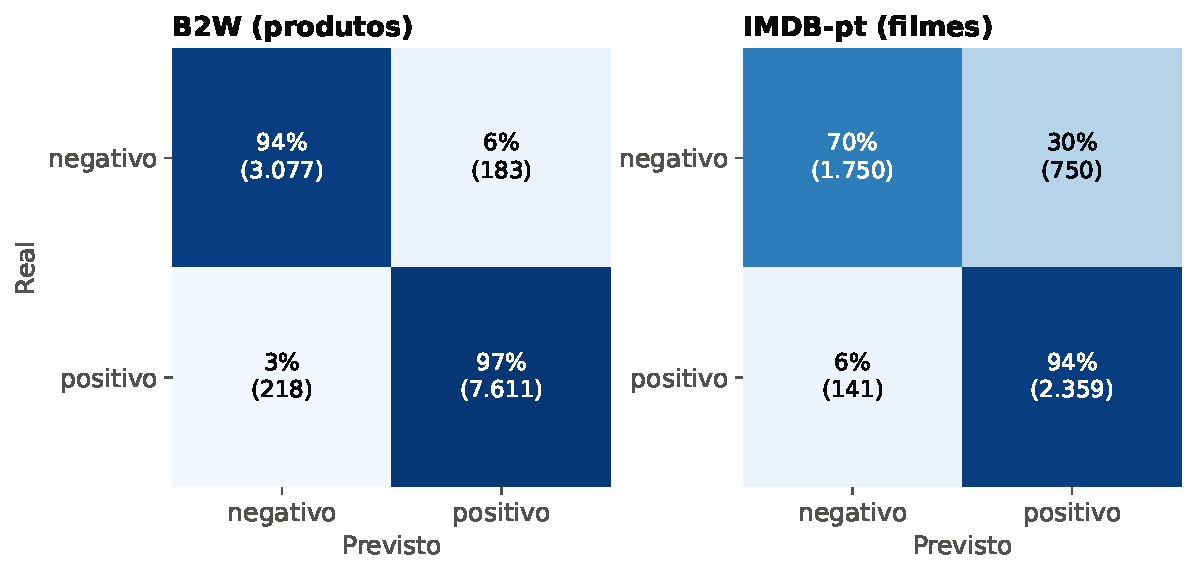
\includegraphics[width=\textwidth]{matrizes_confusao.pdf}
    \end{column}
    \begin{column}{0.42\textwidth}
      \small
      \begin{itemize}
        \item o modelo do E2, sem nenhum exemplo de filme: F1 cai de 95,7\% (produtos) para \alert{81,9\%} (filmes)
        \item erro de um lado só: \alert{30\%} das críticas negativas viram ``positivo'', contra 6\% no sentido oposto
        \item hipóteses: treino com 70\% positivos, críticas longas que misturam elogio e crítica, texto traduzido
        \item mesmo assim, 82\% sem ter visto filmes
      \end{itemize}
    \end{column}
  \end{columns}
  \fonte{E5; IMDB-pt, 5.000 críticas [9]. As hipóteses não foram testadas separadamente.}
\end{frame}

% ===================================================================
% Bloco 8: aplicações, vantagens e limitações (1,5 min)
% ===================================================================

\section{Aplicações, vantagens e limitações}

\begin{frame}{Aplicações}
  \small
  \begin{tabular}{@{}L{0.2\textwidth}L{0.72\textwidth}@{}}
    \toprule
    \textbf{Área} & \textbf{Exemplo} \\
    \midrule
    Comércio eletrônico & sentimento de avaliações (este trabalho): 95,7\% de F1 \\
    Biomedicina & BioBERT: entidades, relações e perguntas e respostas em textos biomédicos [10] \\
    Finanças & FinBERT: sentimento em textos financeiros, com poucos dados rotulados [11] \\
    Direito & LEGAL-BERT: classificação e extração em textos jurídicos [12] \\
    Assistentes & InstructGPT: ajuste fino com demonstrações humanas; o modelo de 1,3 B foi preferido ao GPT-3 de 175 B [13] \\
    \bottomrule
  \end{tabular}
  \vspace{0.8em}

  Os de domínio especializado continuam o pré-treino no texto do domínio \emph{antes} do ajuste fino.
  \fonte{Resumos dos artigos [10]--[13].}
\end{frame}

\begin{frame}{Vantagens e limitações}
  \begin{columns}[T]
    \begin{column}{0.48\textwidth}
      \textbf{\color{azul}Vantagens}
      \begin{itemize}
        \item \textbf{poucos dados}: 1.000 exemplos já superam o TF-IDF com 20.000
        \item \textbf{melhor que o clássico}: erro 46\% menor com os mesmos dados
        \item \textbf{barato}: 4 min e 3 GB numa GPU gratuita
        \item \textbf{mesma receita} para várias tarefas
      \end{itemize}
    \end{column}
    \begin{column}{0.48\textwidth}
      \textbf{\color{laranja}Limitações}
      \begin{itemize}
        \item \textbf{sobreajuste} com poucos dados: exige validação e early stopping
        \item \textbf{mudança de domínio}: $-$14 pontos em filmes
        \item \textbf{confiança enganosa}: ironia errada com 99,6\%
        \item \textbf{instável}: sementes diferentes mudam o resultado [4, 5]
        \item \textbf{custo cresce} com o modelo: uma cópia de todos os pesos por tarefa; daí o LoRA [14]
      \end{itemize}
    \end{column}
  \end{columns}
  \fonte{Experimentos E1--E6; Mosbach et al. [4]; Dodge et al. [5]; Hu et al. [14].}
\end{frame}

% ===================================================================
% Bloco 9: fechamento (0,5 min)
% ===================================================================

\begin{frame}{Resumo}
  \begin{enumerate}
    \item Ajuste fino = modelo pré-treinado + cabeça nova + poucos exemplos rotulados + taxa pequena
    \item O código tem três partes: \textbf{preparar} (rótulo, divisão, tokenização), \textbf{treinar} (\texttt{Trainer}), \textbf{inferir} (\texttt{pipeline})
    \item No exemplo: \destaque{95,7\%} de F1, acima do TF-IDF, em 4 minutos numa GPU gratuita
    \item Sobreajuste aparece cedo com poucos dados; a validação e o early stopping resolvem
    \item Fora do domínio de treino, o desempenho cai: \alert{sempre avaliar onde o modelo vai ser usado}
  \end{enumerate}
  \vspace{1em}
  \centering
  {\large Obrigado! Perguntas?}\\[4pt]
  \small Código e resultados: \texttt{github.com/Aladiah96/trabalho-nlp}
\end{frame}

\begin{frame}{Referências}
  \scriptsize
  \begin{enumerate}
    \item[{[1]}] Devlin, Chang, Lee e Toutanova. BERT: Pre-training of Deep Bidirectional Transformers for Language Understanding. NAACL, 2019.
    \item[{[2]}] Howard e Ruder. Universal Language Model Fine-tuning for Text Classification. ACL, 2018.
    \item[{[3]}] Souza, Nogueira e Lotufo. BERTimbau: Pretrained BERT Models for Brazilian Portuguese. BRACIS, 2020.
    \item[{[4]}] Mosbach, Andriushchenko e Klakow. On the Stability of Fine-tuning BERT. ICLR, 2021.
    \item[{[5]}] Dodge et al. Fine-Tuning Pretrained Language Models: Weight Initializations, Data Orders, and Early Stopping. arXiv:2002.06305, 2020.
    \item[{[8]}] Real, Oshiro e Mafra. B2W-Reviews01: an open product reviews corpus. STIL, 2019.
    \item[{[9]}] Maas et al. Learning Word Vectors for Sentiment Analysis. ACL, 2011. Versão em português: \texttt{maritaca-ai/imdb\_pt}.
    \item[{[10]}] Lee et al. BioBERT: a pre-trained biomedical language representation model for biomedical text mining. Bioinformatics, 2020.
    \item[{[11]}] Araci. FinBERT: Financial Sentiment Analysis with Pre-trained Language Models. arXiv:1908.10063, 2019.
    \item[{[12]}] Chalkidis et al. LEGAL-BERT: The Muppets straight out of Law School. Findings of EMNLP, 2020.
    \item[{[13]}] Ouyang et al. Training language models to follow instructions with human feedback. NeurIPS, 2022.
    \item[{[14]}] Hu et al. LoRA: Low-Rank Adaptation of Large Language Models. ICLR, 2022.
  \end{enumerate}
\end{frame}

\end{document}
